% !Mode:: "TeX:UTF-8" 

\BiChapter{目标识别模型设计及数据集搭建}{2}\label{chpt-2}
本毕设的首要任务是完成图~\ref{fig-introduction}~中竞技场部分的目标识别问题,
因为决策所需的状态信息主要来自于该部分,对于竞技场中第$i$个单位$u_i$,
其所包含的信息可以表示为$u=(\boldsymbol{x}, \text{cls}, \text{bel}, \text{bar}_1, \text{bar}_2)$,
其中$\boldsymbol{x}$表示$u$所在的网格坐标,$\text{cls}$表示$u$所属的部队类别,
$\text{bel}$表示$u$所属的派别,$\text{bar}_1,\text{bar}_2$表示$u$当前的生命值图像及其余条状图像信息。

在本章节将介绍如何使用目标识别模型完成对每个单位中$\boldsymbol{x}, \text{cls}, \text{bel}$信息的识别,
由于训练目标识别模型需要基于大量的有标记图像,而该任务没有任何相关的开源数据集,若逐帧人工标记效率极低且成本高昂,
因此本毕设基于该任务提出一种高效的带标记图像的生成方案,并重构目标识别代码使其可以有效训练该生成式数据集以满足上述识别要求,
相关实验结果在~\ref{sec-exp-data}~中展示。

识别数据集制作以及模型更新流程如图~\ref{fig-annotation}~所示,
其中左上部分的“原视频流”为一个回合的视频数据,若存在之前训练的目标识别模型,则
使用该模型进行对视频流进行辅助标记,获得“辅助标记视频流”再进行手工标记,否则直接对“原视频流”进行手工标记;
在手工标记中,以0.5秒作为标记间隔,进行人工目标框标记;然后将目标框和原图像同时传入到SAM模型当中获取前景分割,
将分割后的结果进行人工筛选获得“切片数据集”;基于已完成的切片数据集,利用生成式数据集算法,对目标识别模型进行迭代更新,
从而用于下一次的辅助标记过程。
\begin{figure}[htbp]
  \centering
  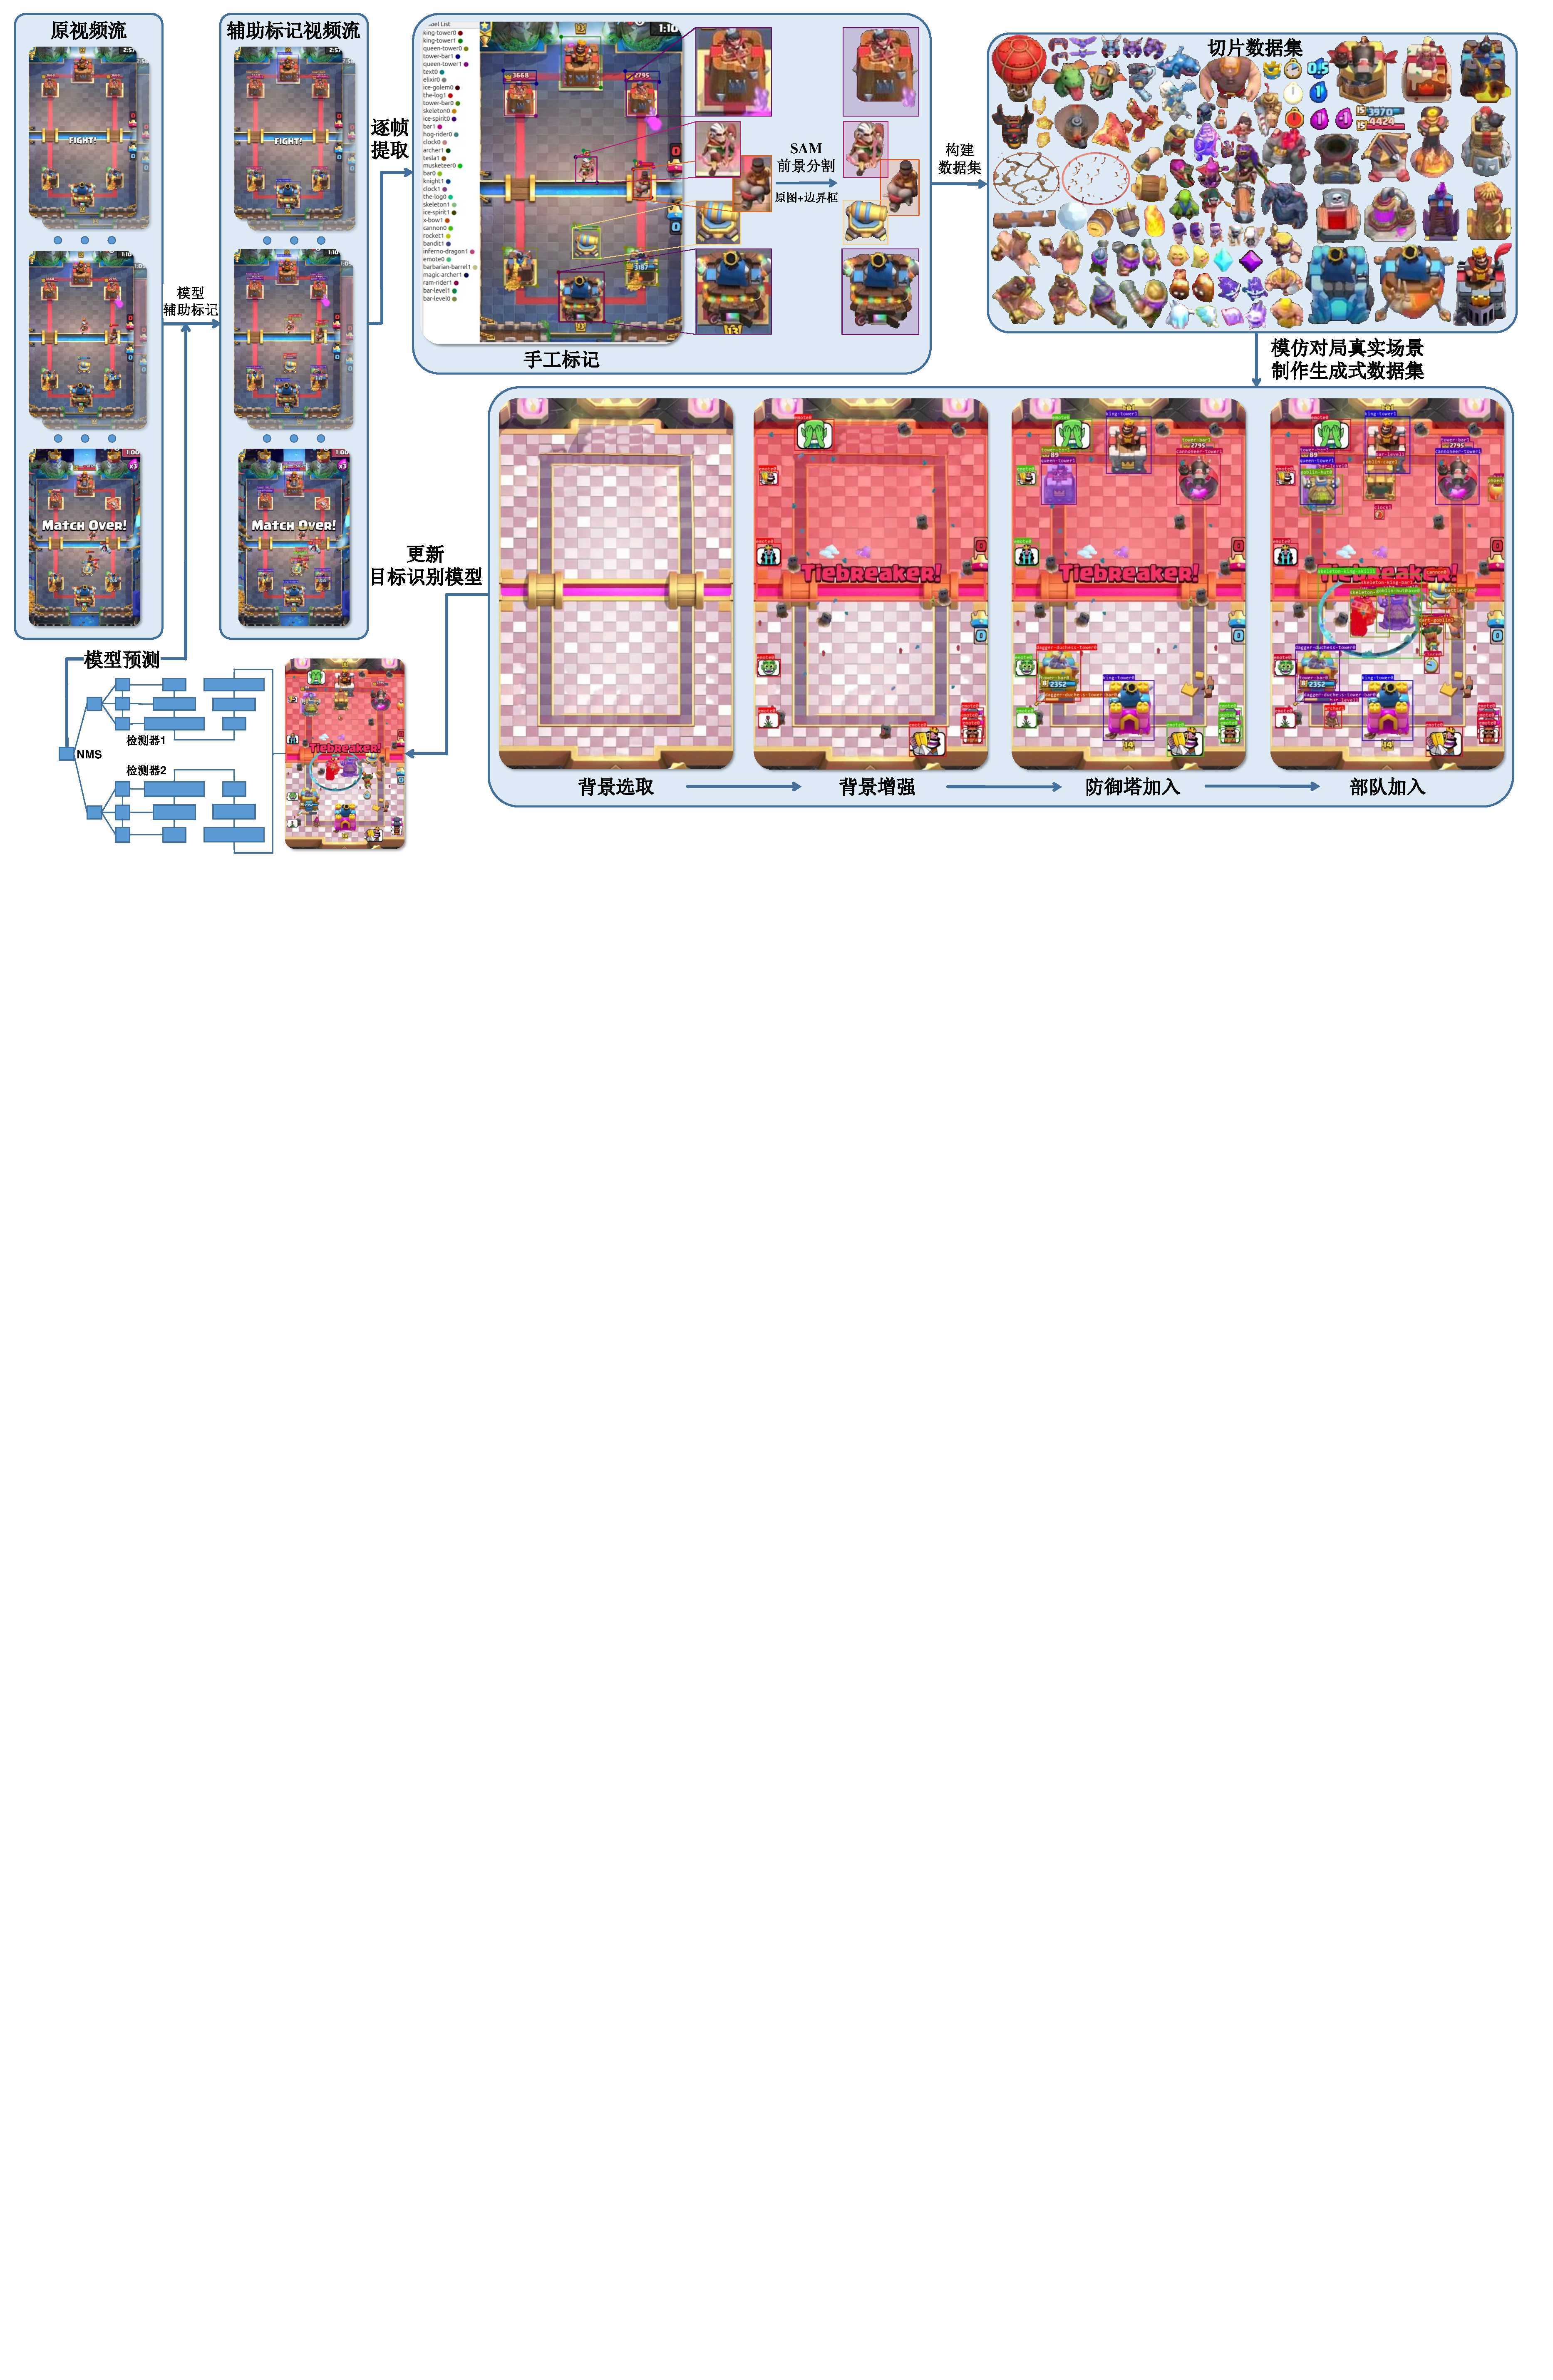
\includegraphics[width=1.0\textwidth]{detection dataset building.pdf}
  \caption{目标识别数据集制作流程}
  \label{fig-annotation}
\end{figure}

\BiSection{切片数据集制作流程}{2-1}
切片数据集中制作本毕设使用了一个强大的通用计算机视觉模型:Segment Anything Model (SAM)\upcite{SAM},该模型为Meta AI公司于2023年开源,
可以根据输入的提示信息生成对象的分割掩码,也可对图像中的所有对象生成掩码,
其是在一个包含1100万张图像和11亿个掩码的数据集上进行训练得到的,能够在很多零样本任务上表现出强大的性能,
SAM模型的核型框架包含如下三个部分:
\begin{enumerate}
  \item 视觉编码器(Vision Encoder):基于ViT的图像特征提取架构,用于捕获图像的上下帧信息,将输入图像转化为特征编码。
  \item 提示编码器(Prompt Encoder):用于处理输入中的提示信息,提示信息分为离散(点、框选区域、文本信息)和连续(掩码)两种,
  分别使用位置嵌入(Positional Encoding)和CNN对提示信息进行编码。
  \item 解码器(Decoder):将视觉编码器和提示编码器生成的特征进行融合,并输出提示信息所对应的分割掩码。
\end{enumerate}

由于生成式数据集需要获取每一个单位不同角度的切片图像,人工创建分割掩码过于繁琐,但单位的目标框相对容易标注,
所以考虑使用SAM中框选区域的提示方式生成对象掩码,图~\ref{fig-annotation}~的中上以及右上部分展示了使用SAM制作切片数据集的过程。

\BiSection{目标识别模型设计}{2-2}
由于需要追求高效的识别速度,所以本文使用了一阶段识别器YOLOv8\upcite{YOLOv8},下面对YOLO系列模型架构进行分析,
并给出本文对其进行修改的部分。

设$x,y,w,h$为正实数,四元组$B=(x,y,w,h)$称为边界框,其中
$(x,y)$表示当前边界框中心,$(w,h)$表示边界框的宽度和高度。

对于任意两个边界框$B_1,B_2$,$S_1,S_2$分别表示其所围住的点集,
则称$B_1,B_2$的交并比(Intersection over Union, IOU)为$\text{IOU}_{B_2}^{B_1}:=\frac{S_1\cap S_2}{S_1\cup S_2}$。

设$S,B,C\in\mathbb{Z}^+$分别表示图像网格化大小、每个网格中边界框预测框数目、总分类类别数,通过CNN可以将图像空间进行压缩,
从而得到对应的不同网格化大小。例如,在如图~\ref{fig-anchor}~中原图像宽高为$416\times 416$,CNN中每次降采样会将图像的宽高均减小一半,
于是经过步长(Stride)为$s=2^3$的降采样就可以得到左图中$(H/s)\times (W/s) =: S\times S$即$52\times 52$的网格大小,
每个网格中的感受野大小(即步长)即为对应网格中$2^3\times 2^3$个像素,
目标识别模型需要在每个网格处做出$B$个边界框框预测。

图~\ref{fig-anchor}~中,对于每个目标框$B$,其中心点用黄色点标出,假设该中心点位于网格大小为$52\times 52$中的第$(i,j)$网格内,
则在模型预测的输出中,也应该由$(i,j)$网格对应的边界框进行预测。在YOLOv3\upcite{YOLOv3}中,将Fast-RCNN\upcite{FastRCNN}中锚框的概念引入YOLO系列,
对于不同的网格划分,对应分配不同的尺度估计框,称为锚框(Anchor Bounding Box),
这些锚框是基于数据集中的全体锚框做K近邻得到(距离衡量标准为负的相对交并比),该方法可以将数据集中识别框大小的先验信息引入到模型中。
按照网格划分的从大到小,分别分配$B$个从小到大的锚框,
因为更大的网格对应更高的分辨率,其具有更多的细节信息,从而可以识别小目标框,
所以给其分配更小的锚框,反之亦然。

\begin{figure}[htbp]
  \centering
  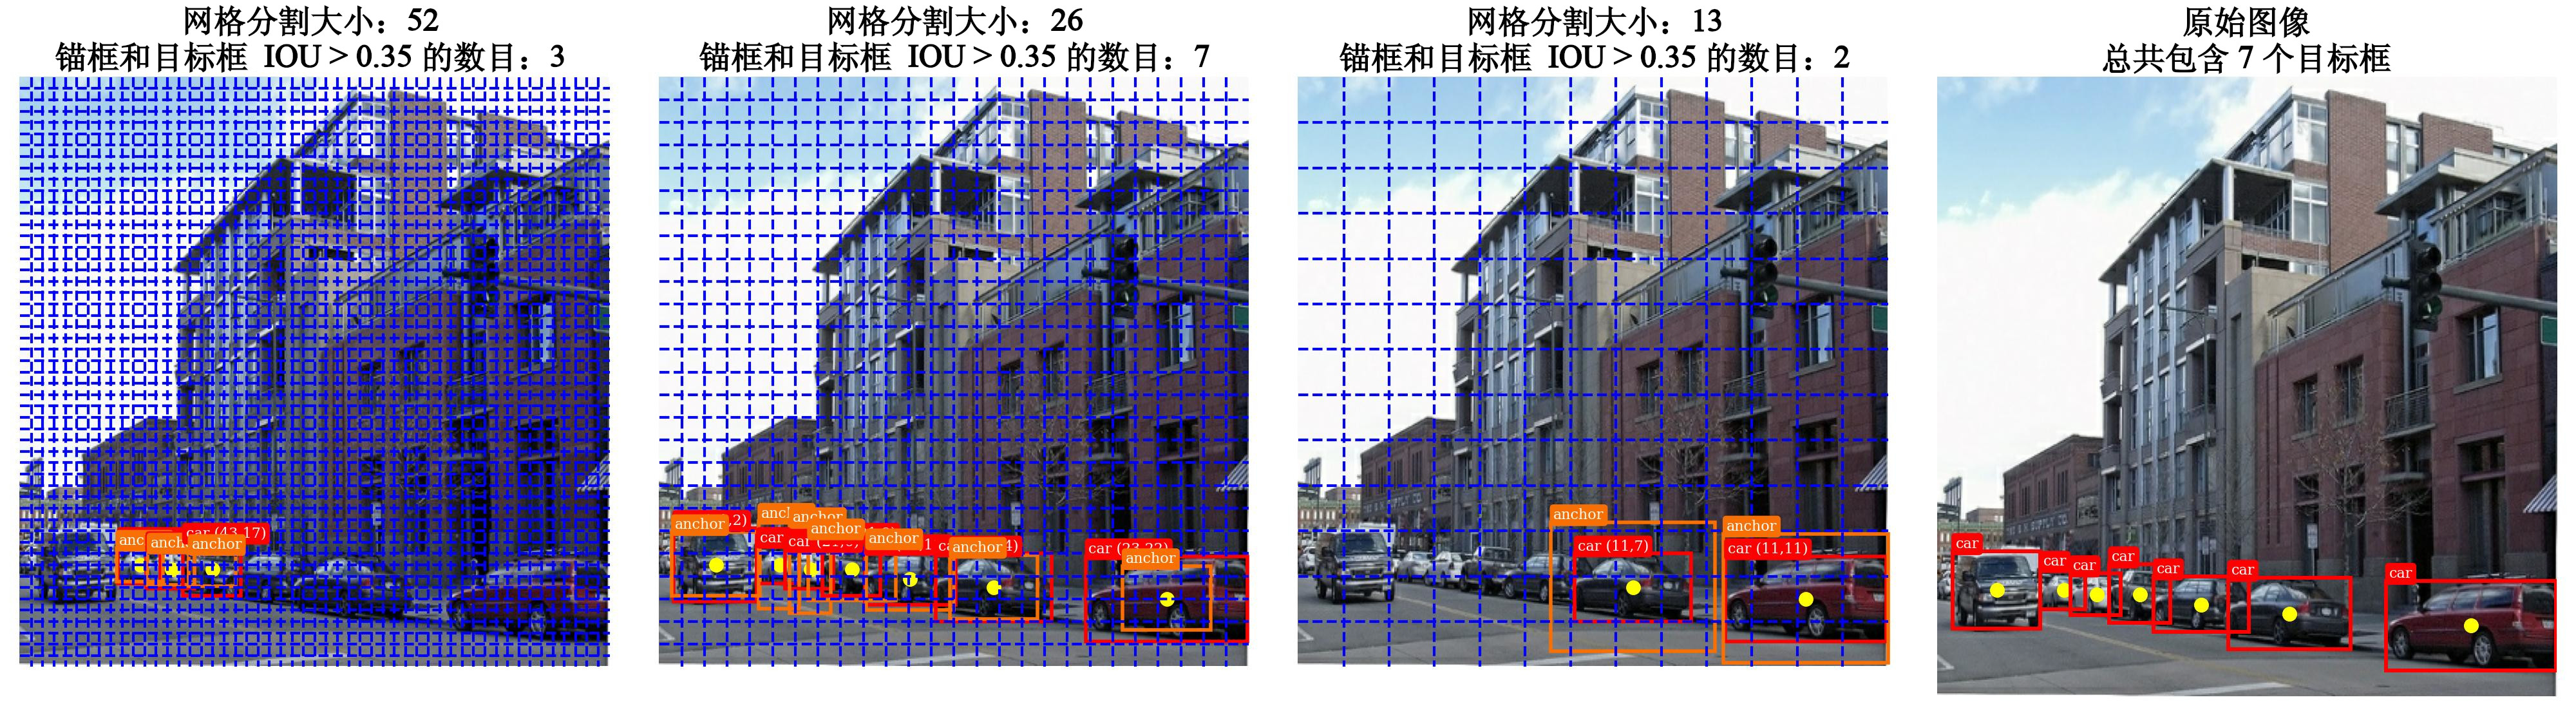
\includegraphics[width=\textwidth]{yolo_anchor_box.jpg}
  \caption{3个不同网格大小下的目标框与锚框,红色为目标框,橙色为基于数据集分配的锚框,
  在3个不同的网格大小下各分配了3种锚框,在图中只显示了相对$\text{IOU}>0.35$的锚框。
  演示的标记图片来自于PASCAL VOC数据集\upcite{PascalVOC},图像大小为$416\times 416$。}
  \label{fig-anchor}
\end{figure}

假设当前网格步长为$s$,对应的一个锚框为$(A_w,A_h)$,则网格$(i,j)$处的相对预测框定义为六元组$(x,y,w,h,c,\{p_c\}_{c=1}^C, \text{bel})$,其中:
\begin{itemize}
  \item $(x,y)$表示当前预测框中心点相对于步长$s$的比例,偏移量为$(i\cdot s, j\cdot s)$。
  \item $(w,h)$表示当前预测框的长宽相对于锚框$(A_w,A_h)$的比例。
  \item $c$表示当前预测的置信度,定义为$\text{Pr}(\text{Object})\cdot \text{IOU}_{pred}^{true}$。
  \item $p_c$表示当前预测框预测为类别$c$的概率。
  \item $\text{bel}$表示当前预测框预测从属派别为敌方的概率。
\end{itemize}
不难看出,当前网格步长$s$下网格$(i,j)$处的相对预测框所对应的全局边界框为$((j+x)s,(i+y)s, wA_w, hA_h)$。
传统目标识别通常为单类别识别,本毕设任务由于包含单位的从属派别类别,故为多类别识别问题,需要对预测结果以及对应损失函数进行修改。

设模型的输出为$\hat{\bd{z}}\in\mathbb{R}^{N}$,则模型预测分布为(Softmax变换)
\begin{equation}
  \hat{\bd{y}}_i = \text{softmax}(\bd{z})_i = \frac{\e^{z_i}}{\sum_{j=1}^N\e^{z_j}}
\end{equation}
对于$N$维离散目标分布为$\bd{y}\in\mathbb{R}^N$,多元交叉交叉熵损失(Cross-Entropy Loss, CE Loss)为
\begin{equation}\label{eq-ce}
  \mathcal{L}_{\text{CE}}(\hat{\bd{y}},\bd{y}) = -\sum_{i=1}^Ny_i\log\hat{y}_{i}
\end{equation}

特殊地,当$N=2$时,不妨令目标分布为$\{y, 1-y\}$,则式~(\ref{eq-ce})~被称为二元交叉熵损失(Binary Cross-Entropy Loss, BCE Loss)
\begin{equation}
  \mathcal{L}_{\text{BCE}}(\hat{\bd{y}},\bd{y}) = y\cdot \log\hat{\bd{y}}_{1} + (1-y)\cdot \log\hat{\bd{y}}_2
\end{equation}

在目标识别任务中目标分布$y$通常为独热分布(Onehot),其中正确预测的概率为$1$,其余类别概率为$0$,
可以表示$\text{onehot}(c) = \{[i=c]\}_{i=1}^C$,$[\text{条件}]$表示当内部条件成立时为$1$,否则为$0$。
然而上述Softmax函数只有当$z_i\gg z_j(i\neq j)$时接近该分布,这会导致模型对其预测过于自信,在目标识别任务中容易出现过拟合现象\upcite{BagFreebiesForObjectDetection}。

设当前网格步长为$s$,输入图像的大小为$W\times H$,每个网格处所需的预测框数目为$B$,\vspace{0.5ex}
第$i$行$j$列网格预测出的第$k$个预测框记为$\left(\widehat{\text{box}}_{ijk},\hat{c}_{ijk}, \hat{p}_{c_{ijk}}, \widehat{\text{bel}}_{ijk}\right)$,
对应的目标框$\left(\text{box}_{ijk}, \text{cls}_{ijk}, \text{bel}_{ijk}\right)$,\vspace{0.5ex}
下面给出该步长下的损失函数
\begin{equation}
\begin{aligned}
\mathcal{L}_{s}(\hat{y}, y) = 
\sum_{i=1}^{H/s}\sum_{j=1}^{W/s}\sum_{k=1}^B&\ \mathbbm{1}^{noobj}_{ijk}\lambda_{noobj}\mathcal{L}_{\text{BCE}}(\hat{c}_{ijk},0)\\
&\ +\mathbbm{1}^{obj}_{ijk}\bigg[\lambda_{\text{box}}\mathcal{L}_{\text{CIOU}}\left(\widehat{\text{box}}_{ijk},\text{box}_{ijk}\right)+
\lambda_{obj}\mathcal{L}_{\text{BCE}}\left(\hat{c}_{ijk},\text{IOU}_{pred}^{true}\right)\\
&\ \qquad\qquad+\lambda_{class}\sum_{c=1}^{C}\mathcal{L}_{\text{BCE}}\bigg(\left\{\hat{p}_{ijk}\right\}_c, \text{onehot}\left(\text{cls}_{ijk}\right)_c\bigg)\\
&\ \qquad\qquad+\lambda_{class}\mathcal{L}_{\text{BCE}}\left(\widehat{\text{bel}}_{ijk}, \text{bel}_{ijk}\right)\bigg]
\end{aligned}
\end{equation}
其中$\mathbbm{1}^{noobj}_{ijk}$当网格$(i,j)$下的第$k$个预测框没有对应的目标框时为$1$,反之为$0$,
相反的$\mathbbm{1}^{obj}_{ijk} = 1-\mathbbm{1}^{noobj}_{ijk}$,
$\mathcal{L}_{\text{CIOU}}$为Complete-IOU损失\upcite{CIOU}是基于IOU损失的一种改进,边界框回归预测问题中相比MSE损失能够更快地收敛。

由于本任务的类别数目超过150种,而当前通用目标识别数据集COCO\upcite{COCO}类别仅为80种,所以本文使用了双模型识别器,如图~\ref{fig-annotation}~中左下角部分,
多个检测器进行组合的模型预测效果见第五章中表~\ref{tabel-yolo}。

\BiSection{生成式目标识别数据集}{2-3}
假设将每个切片作为绘制单位,定义$u = (img,box,level)$,其中$img$为绘制单位的切片图像;
$box=(x,y,w,h,\text{cls},\text{bel})$为绘制单位的边界框参数,$(x,y)$为切片中心点位于图像的二维坐标,
$(w,h)$为切片的宽高大小,cls为当前切片的所属类别,bel为当前切片的所属派别;$level$为当前切片的所属图层等级,
图层等价划分如表~\ref{tab-level}~所示。
\begin{table}[htbp]
	\renewcommand{\arraystretch}{1.2}
	\centering\wuhao
	\caption{图层等级与切片类别关系表} \label{tab-level} \vspace{2mm}
	\begin{tabularx}{\textwidth} { 
   >{\centering\arraybackslash\hsize=.6\hsize}X 
   >{\centering\arraybackslash}X }
	\toprule[1.5pt]
		图层等级 & 切片类别 \\
	\midrule[1pt]
		0 & 地面法术,地面背景部件 \\
		1 & 地面部队,防御塔 \\
		2 & 空中部队,空中法术 \\
		3 & 其余待识别部件,空中背景部件 \\
	\bottomrule[1.5pt]
	\end{tabularx}
\end{table}

绘制单位的插入流程如图~\ref{fig-annotation}~中右下角部分所示,具体细节如下:
\begin{enumerate}
  \item 背景选取:从数据集中随机选取一个去除防御塔、部队及文本信息的空竞技场作为背景图片。
  \item 背景增强:加入背景板中的非目标识别部件,用于数据增强,例如:部队阵亡时的圣水,场景中随机出现的蝴蝶、花朵等。
  \item 防御塔加入:在双方的三个防御塔固定点位上随机生成完好或被摧毁的防御塔,并随机选取生成与之相关联的生命值信息。
  \item 部队加入:按照类别出现次数的反比例$\left\{\frac{1}{n_{c_i}-n_{\min}+1}\right\}_{i=1}^{|C|}$\vspace{0.5ex}
  所对应的分布进行类别随机选取,其中$n_{c_i},(c_i\in C)$表示类别$c_i$的切片之前生成的总次数,
  $n_{\min}=\min\{n_{c_i}\}_{i=1}^{|C|}$;在竞技场中按照动态概率分布(具体见附录~\ref{app-dynamic-distrib})随机选择生成点位,
  并随机选取生成与之相关的等级、生命值、圣水、时钟等信息。
\end{enumerate}

\begin{algorithm}[ht]
	\caption{生成算法伪代码\label{alg-generator}}
	\IncMargin{2em}
	\DontPrintSemicolon
	\KwIn{绘制单位序列$U=\{u_i\}$,覆盖率阈值$\alpha$,待识别类别集合$C$}
	\KwOut{image, box}
  $\text{image}\gets$空图像,$\text{box}\gets \{\}$\tcp*{初始化参数}
  $U\gets \{u_i\in U: u_i^{level}>u_j^{level}, \forall i, j \in \{1,\cdots,|U|\} \text{~且~} i < j\}$\;
  \While{True}{
    $\text{mask}\gets$空掩码,$U_{avail}\gets U$\;
    \For{$i=1,2,\cdots,|U|$}{
      \If{$\frac{u^{img}_i\cap~ \text{mask}}{u_i^{img}} > \alpha$}{
        $U_{avail}\gets U_{avail} - R(u_i)$\tcp*{删除与$u_i$相关联的单位}
      }
      $\text{mask}\gets \text{mask}\cup u_i^{img}$\;
    }
    \If{$|U_{avail}|=|U|$}{
      break\tcp*{覆盖单位筛选完成}
    }
    $U\gets U_{avail}$
  }
  $U\gets \{u_i\in U: u_i^{level}<u_j^{level}, \forall i, j \in \{1,\cdots,|U|\} \text{~且~} i < j\}$\;
  \For{$i=1,2,\cdots,|U|$}{
    $\text{img}\gets \text{img} \cup u_i^{img}$\tcp*{图像绘制}
    \If{$u_{i}^{\text{cls}}\in C$}{
      $\text{box}\gets \text{box} \cup u_i^{box}$\tcp*{边界框保存}
    }
  }
\end{algorithm}
\newpage
完成绘制单位加入后,可以按照插入顺序得到待绘制单位序列$U$,但生成的切片可能存在覆盖关系,因此需要引入最大覆盖率阈值$\alpha$,
当被覆盖单位面积超过该单位切片面积的$\alpha$倍时,对被覆盖单位进行去除,对单位完成筛选之后,
再按照图层等级的从高到低进行绘制,并将识别类别$C$中的边界框信息进行记录,用于后续识别模型训练,
具体绘制流程见算法~\ref{alg-generator}。% 通过该生成式算法得到的带标签图像如图~\ref{fig-generation}~所示。
通过调整不同的单位生成数量、切片生成类型,最大覆盖阈值$\alpha$,可以得到如图~\ref{fig-generation}~所示的生成结果,
生成式代码框架见附录~\ref{app-generator}。

\begin{figure}[h!]
\centering\vspace{-0.0ex}
\subfigure[单位生成数量20,小型切片类型,$\alpha=0.5$]{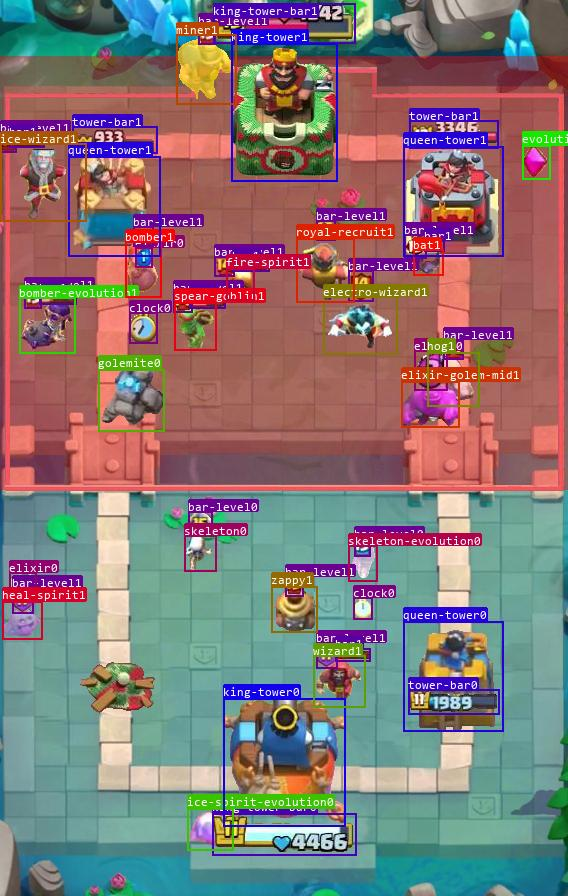
\includegraphics[width=0.32\textwidth]{generation/nu20,small,0.5.jpg}}
\subfigure[单位生成数量20,大型切片类型,$\alpha=0.5$]{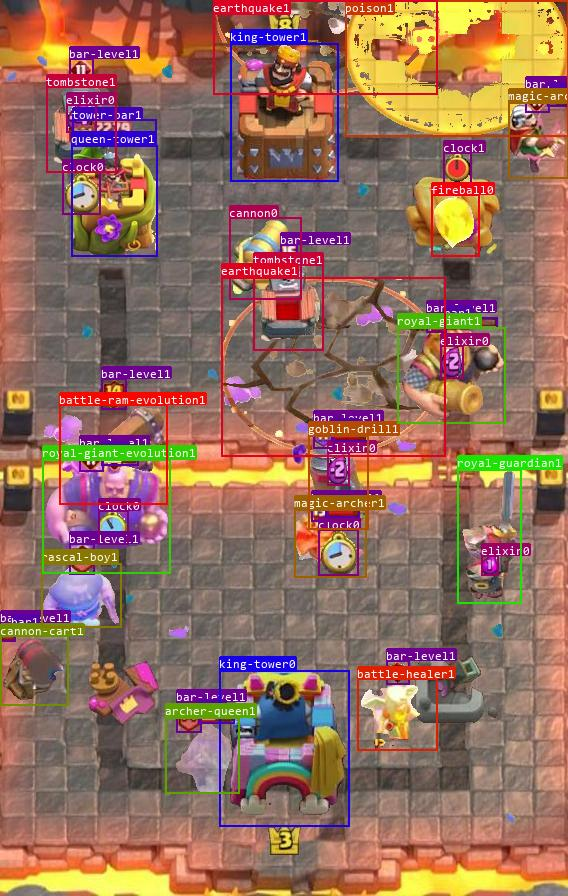
\includegraphics[width=0.32\textwidth]{generation/nu20,big,0.5.jpg}}
\subfigure[单位生成数量20,大型切片类型,$\alpha=0.8$]{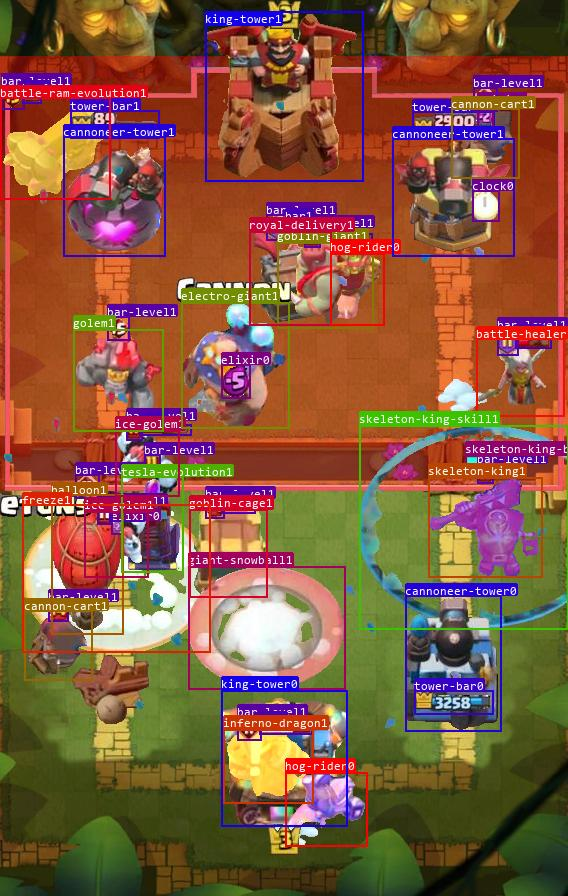
\includegraphics[width=0.32\textwidth]{generation/nu20,big,0.8.jpg}}
\subfigure[单位生成数量40,小型切片类型,$\alpha=0.5$]{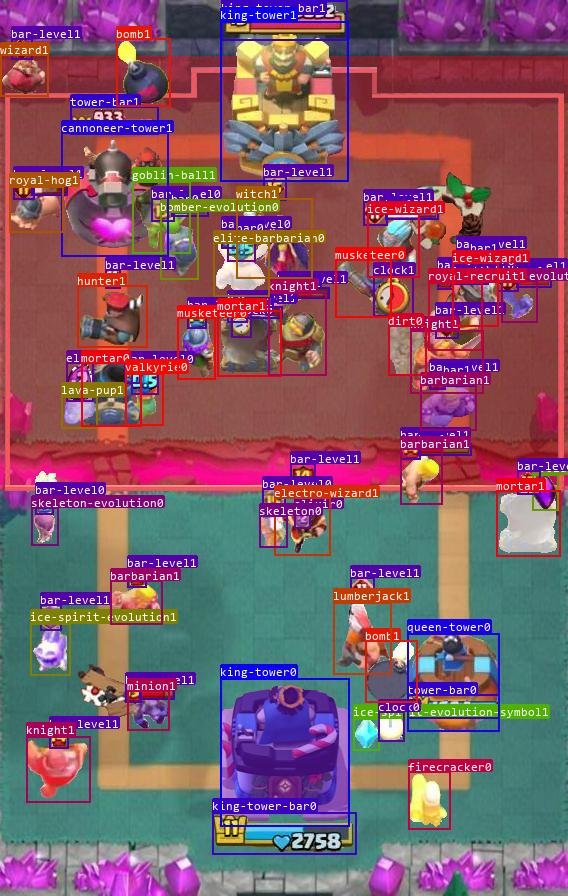
\includegraphics[width=0.32\textwidth]{generation/nu40,small,0.5.jpg}}
\subfigure[单位生成数量40,大型切片类型,$\alpha=0.5$]{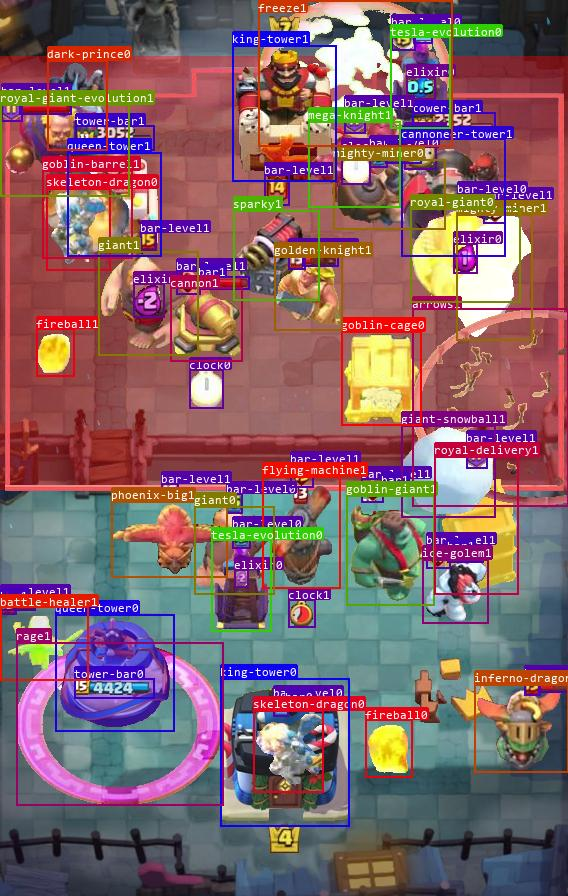
\includegraphics[width=0.32\textwidth]{generation/nu40,big,0.5.jpg}}
\subfigure[单位生成数量40,大型切片类型,$\alpha=0.8$]{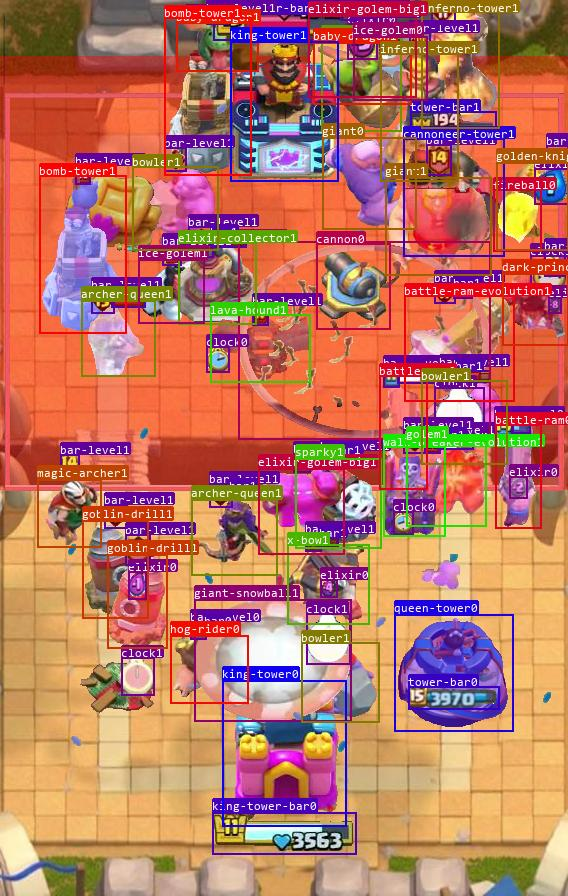
\includegraphics[width=0.32\textwidth]{generation/nu40,big,0.8.jpg}}
\setlength{\abovecaptionskip}{0ex}  % 由于minted会增大图像与标题间距需要进行缩小
\caption{生成式数据集实例}\label{fig-generation}
\end{figure}

\BiSection{本章小结}{}
本章介绍了使用目标识别模型完成对每个单位识别的方法,设计了相应的损失函数,并给出了一种制作生成式数据集切片的方法,
基于该方法制作了用于目标识别模型训练的生成式数据集(数据集分析与统计信息见~\ref{sec-exp-data}),
还通过对视频流数据集逐帧进行人工标记,制作了用于测试模型性能的验证集。

本章设计了双模型以及三模型的模型组合方式,使用生成式数据集训练模型,
再在验证集中进行验证,全部模型均表现出良好的泛化能力,
其中最好的模型在验证集中达到了$68.8\%$~mAP指标并在$50\%$交并比阈值下达到了$80.9\%$召回率,
同时保持每张图片$43$毫秒的实时推理性能(模型验证结果见表~\ref{tabel-yolo})。
